\chapter{Reporting Errors}
\label{user-errors}

If \FramaC crashes or behaves abnormally, you are invited to report a bug \via
the \FramaC Bugs Tracking System (BTS) located at
\url{http://bts.frama-c.com}. 

\begin{important}
Opening a BTS account is required for such a task. 
\end{important}

Bug reports can be marked as public or private.
Public bug reports can be read by anyone and are indexed by search
engines. Private bug reports are only shown to \FramaC developers. 

Reporting a new issue opens a webpage similar to the one shown in
Figure~\ref{fig:bts}.
\begin{figure}[htbp]
\begin{center}
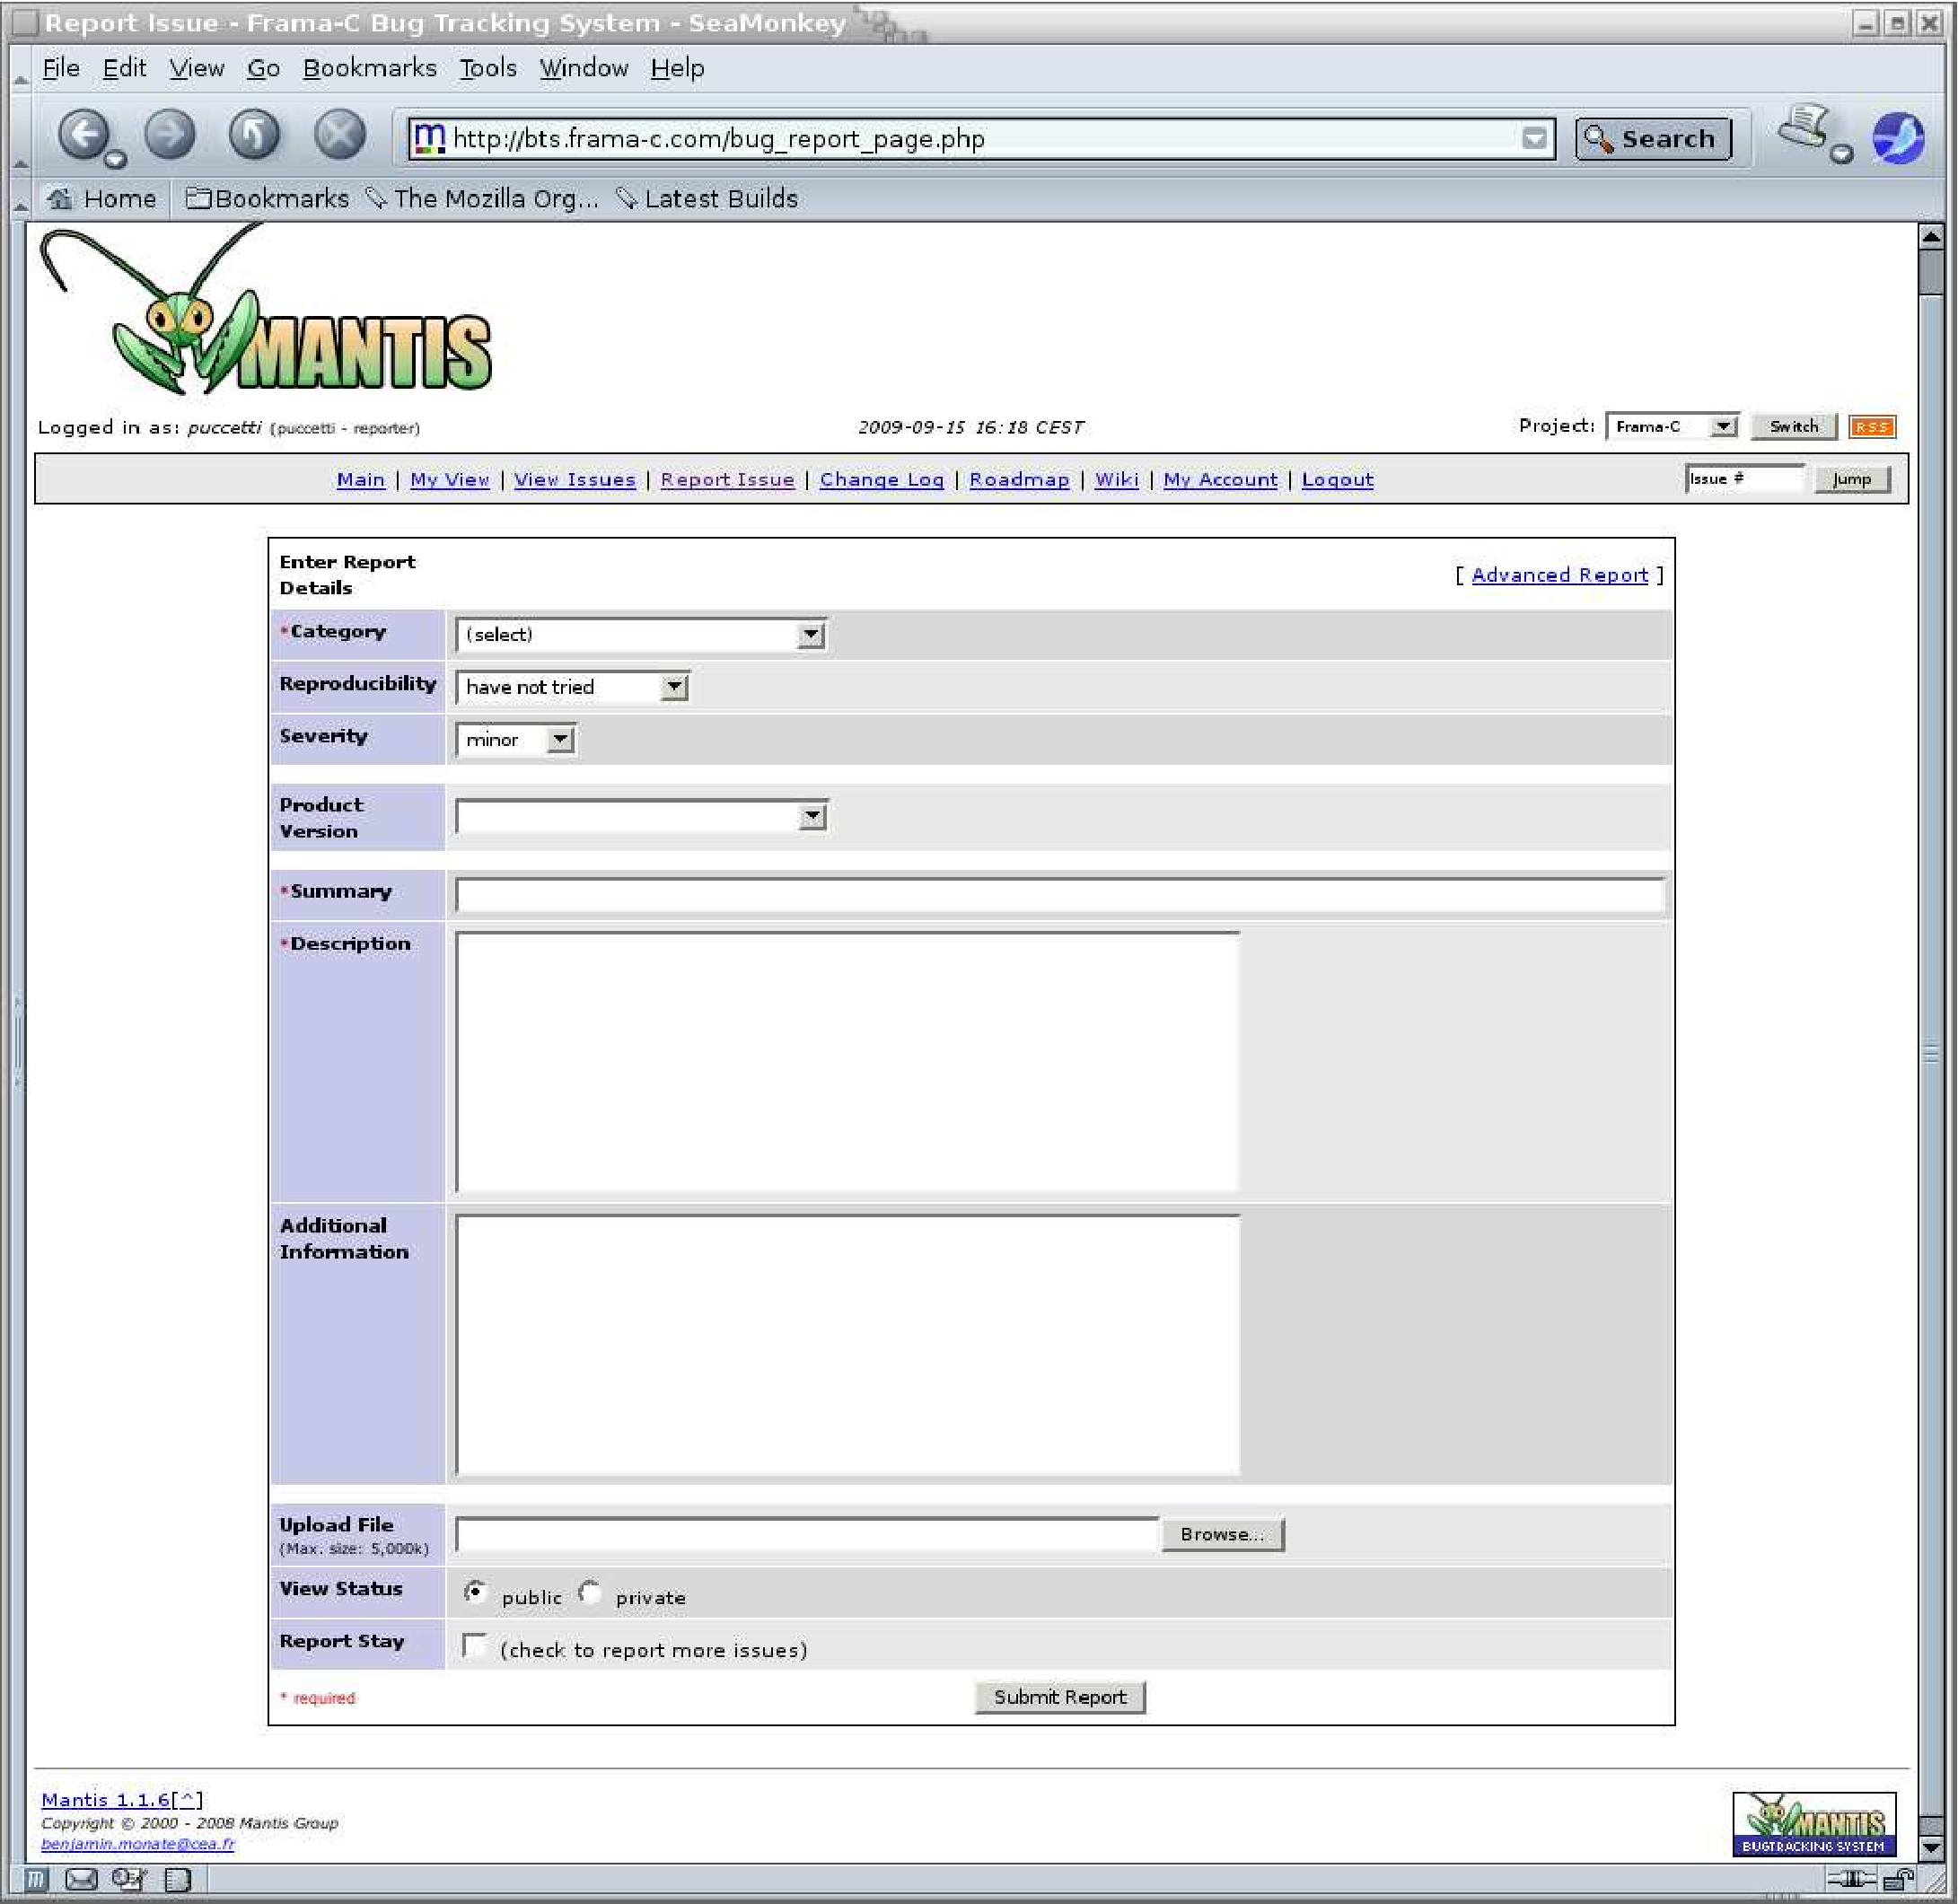
\includegraphics[width=\textwidth]{bts.pdf}
\end{center}
\caption{The BTS Bugs Reporting Page}
\label{fig:bts}
\end{figure}
This page also has a link to an advanced bugs reporting page that allows you to
write a more detailed report. The different fields of these forms shall be
filled \emph{in English}\footnote{French is also a possible language choice for private entries.}
as precisely as possible, in order for the maintenance team to understand and
track the problem down easily.

Below are some recommendations for this purpose\footnote{You can also have a
  look at the associated \FramaC wiki:
  \url{http://bts.frama-c.com/dokuwiki/doku.php?id=mantis:frama-c:start}.}:

\begin{description}

\item[Category:] select as appropriate.

\item[Reproducibility:] select as appropriate.

\item[Severity:] select the level of severity. Levels are shown in increasing
  order of severity.

\item[Profile or Platform, OS and OS Version:] enter your hardware and OS
  characteristics.

\item[Product Version and Product Build] this can be obtained with the
  command \texttt{frama-c -version}\optionidx{-}{version}, see
  Section~\ref{sec:version}.

\item[Summary:] give a brief one line description of the nature of your bug.

\item[Description:] first, explain the \textit{actual behavior}, that is what
  you actually observe on your system. Then, describe your \textit{expected
    behavior} of \FramaC, that is the results you expect instead. A ``bug'' is
  sometimes due to a misunderstanding of the tool's behaviour or a
  misunderstanding of its results, so providing both behaviors is an essential
  part of the report. Please do clearly separate both parts in the description.

\item[Steps to reproduce:] provide everything necessary for a maintainer to
  reproduce the bug: input files, commands used, sequence of actions, \etc.  If
  the bug appears through the \FramaC GUI, it may be useful to attach the
  generated journal (see Section~\ref{sec:journal}). Beware that this journal
  \textbf{does not} replace nor contain the input files, that must be added to
  the bug report too (see below).

\item[Additional Information:] any extra information that might help the
  maintainer.

\item[Industrial:] set it to \texttt{true} if you have a maintenance contract
  with the \FramaC development team.

\item[Upload File:] click on the \texttt{Browse} button to select a file for
  uploading.  Typically, this is an archive that contains all files necessary
  for reproducing your problem. It can include \C source files, shell scripts
  to run \FramaC with your options and environment, a \FramaC journal,
  \etc. Please check the size of the archive in order to keep it manageable:
  leave out any object code or executable files that can be easily rebuilt
  automatically (by a shell script for instance).

\item[View Status:] set it to \texttt{private} if your bug should not be
  visible by others users. Only yourself and the \FramaC developers will be
  able to see your bug report.

\item[Report Stay:] tick if this report shall remain open for further
  additions.

\end{description}

After submitting the report you will be notified by e-mail about its progress
and enter interactive mode on the BTS if necessary.

%% Local Variables:
%% compile-command: "make"
%% TeX-master: "userman.tex"
%% ispell-local-dictionary: "english"
%% End:
